\section{Model}

The model follows a discrete timing and embeds 4 types of agents; the households, the firms, the fiscal authority and the central bank. Households can be unemployed or employed through a fixed-term or an open-ended contract. Three types of firms coexist. Perfectly competitive firms produce the final good valued by households for consumption and investment. Final good producers aggregate the differentiated goods produced by the retailers. The latter retailers are in monopolistic competition and transform the homogeneous intermediate good into a differentiated retail good. Intermediate firms produce the associated intermediate good and experience perfect competition. These intermediate firms use labor as their only input. I now describe the behavior of different types of agents in more detail.

\subsection{Households}

Households are identical and constitute a continuum represented  by the interval $(0,1)$. They can be employed under a fixed-term or an open-ended contract, or unemployed. They earn wages or unemployment benefits accordingly. Households also hold firms, consume the homogeneous good produced by final good firms, save using one-period nominal bonds, earn interests on their savings and pay lump-sum taxes. Hence, I assume that taxes do not distort the choice of households over consumption and investment. I do not consider the interplay between payroll taxes and labor market dualism.

If households are identical \emph{ex ante}, their different employment histories make them heterogeneous \emph{ex post}. How labor market dualism impacts the consumption and saving behavior of households is beyond the scope of this paper. As \citet{merz1995search} and \citet{andolfatto1996business} first did, I assume that households pool revenues and that capital markets are perfect. Thereby, I rule out the complication heterogeneity brings on. Households share equal consumption and investments. This assumption is not innocuous: unemployed, open-ended and fixed-term workers have different borrowing constraints and \citet{10.2307/43551457} shows that assets shape the search behavior. I leave these issues for future research. 

The household's program boils down to

\begin{align*}
&\max_{\left\{c_t, B_{t+1} \right\}_{t=0}^{+\infty}} \mathbb{E}_0 \sum_{t = 0}^{+\infty} \beta^t u\left(c_t\right)\\
&\text{s.t} \quad c_t + \frac{B_{t+1}}{P_t} = R_{t-1} \frac{B_{t}}{P_t} + \overline{w_t^p} n_t^p + \overline{w_t^f} n_t^f + \rho^b \overline{w_t} u_t + \Pi_t - \tau_t
\end{align*}

$C_t$ marks down consumption. $B_{t}$ is the amount of nominal bond holdings at the beginning of period $t$, with the associated nominal interest rate $R_t$ between $t$ and $t+1$. $\overline{w_t^p}$, $\overline{w_t^f}$ and $\overline{w_t}$ denote respectively the average real wages for open-ended jobs, temporary jobs and all workers. $\rho^b$ denotes the replacement rate of unemployment benefits over the average wage. $n_t^p$ is the aggregate open-ended employment and $n_t^f$ denotes its fixed-term counterpart. $u_t$ marks down the measure of unemployed households. Firms transfer their profits to households through $\Pi_t$, while the government taxes $\tau_t$ to finance the payment of unemployment benefits.

The first order conditions with respect to $c_t$ and $B_{t+1}$ lead to the following Euler equation

\begin{equation}
u' \left( c_t \right) = \beta \mathbb{E}_t \left[ R_{t} \frac{P_t}{P_{t+1}} u' \left( c_{t+1} \right) \right] \label{eq:euler_eq}\\
\end{equation}

As households own firms, the firms' discount factor is $\beta_{t,s} = \beta^{s-t} u' \left( c_s \right) / u' \left( c_t \right)$.

\subsection{Final good firms}

Final good firms are identical and compete to produce the good consumed by households. They use a Dixit-Stiglitz aggregator as technology to put together retail goods and produce $Y_t$.

\begin{equation}
Y_t = \left( \int_{0}^{1} Y_{i,t}^{\frac{\epsilon - 1}{\epsilon_t}} di \right)^{\frac{\epsilon}{\epsilon} - 1} \label{con_fin}
\end{equation}

where $\epsilon$ is the elasticity of substitution between retail goods.

The firm takes as given the price of the retail goods $P_{i,t}$ and the price of the final good $P_t$ and maximizes its profits with respect to the components of its input $\left\{Y_{i,t}\right\}_{i\in(0,1)}$ under the constraint \eqref{con_fin}. The program of the final good firm boils down to

\begin{align*}
&\max_{\left\{Y_{i,t}\right\}_{i\in[0,1]}} P_t Y_t - \int_{0}^{1} P_{i,t} Y_{i,t} di\\
&\text{subject to \eqref{con_fin}}
\end{align*}

The subsequent first order condition provides an expression for the demand of the retail good $i$

\begin{equation}
Y_{i,t} = \left( \frac{P_{i,t}}{P_t} \right)^{-\epsilon} Y_t \label{eq:ret_dem}
\end{equation}

\subsection{Retailers}

Retailers buy goods from intermediate firms and sell the obtained production to final good producer\footnote{At this step, it is possible to introduce capital to extend the model.}. They are in monopolistic competition and lie on the interval $(0,1)$. Retailers accomplish the one-to-one transformation of the intermediate good into a retail good. Denoting $X_{i,t}$ the retailer's input in the intermediate good, the production technology writes

\begin{equation*}
Y_{i,t} = X_{i,t}
\end{equation*}

As a result, retailers face a real marginal cost that equals the relative price of the intermediate good $\phi_t$. I assume that retailers adjust prices as \citet{calvo1983staggered} describe.

\begin{align*}
P_{i,t} = \left\{ \begin{array}{ll}
P_{i,t-1} & \text{ with probability } \psi\\
P_{i,t}^* & \text{ with probability } 1-\psi\\
\end{array}
\right.
\end{align*}

A fraction $\psi$ of retailers is able to adjust its prices to the optimal value $P_{i,t}^*$, whereas the  remaining retailers stick to their former prices. There is no indexation of non-adjusted princes on inflation in this model. The price-setting retailer $i$ at period $t$ has the following program

\begin{align*}
&\max_{P_{i,t}^*} \mathbb{E}_{t} \sum_{T = t}^{+\infty} \beta_{t,T} \psi^{T-t} \left( \frac{P_{i,t}^*}{P_T} - \phi_{T} \right) Y_{i,T} \\
&\text{ subject to } Y_{i,T} = \left( \frac{P_{i,t}^*}{P_T} \right)^{-\epsilon_T} Y_T
\end{align*}

This leads to the following first order condition

\begin{equation}
\mathbb{E}_{t} \sum_{T = t}^{+\infty} \beta_{t,T} \psi^{T-t} P_T^{\epsilon_T} Y_T \left( \frac{P_{i,t}^*}{P_T} - \mu \phi_T \right) = 0 \label{eq:price_eq}
\end{equation}

where $\mu = \epsilon /(\epsilon-1)$ is the mark-up of retailers.

\subsection{Intermediate good firms and the labor market}

Intermediate-good firms use labor as input. They can employ one worker or maintain one vacancy. Workers can be unemployed or employed under a fixed-term or an open-ended contract. They are identical. There is no on-the-job search, which implies that only unemployed workers search for a job. When a firm and a worker meet, the idiosyncratic productivity of the match $z$ is revealed. I assume that idiosyncratic productivity is i.i.d across time and drawn from a distribution with cumulative distribution function $G$. I reluctantly make this assumption for the sake of simplicity. With persistent idiosyncratic productivity, the computation of the equilibrium requires keeping track of the productivity distribution of matches as a state variable. Since the literature considering cycles and dual labor market is in early stages, I prefer to leave the distributional issues for future research. 

The number of firm-worker contacts per period is $m(e,v)$, where $e$ is the number of job-seekers and $v$ is the number of vacancies. A classic measure of the matching activity is the labor market tightness $\theta =  v/e$. The matching function $m$ has constant returns to scale, which enables the definition of the firm-worker meeting probability $p(\theta)$ on the job seekers' side and its counterpart $q(\theta)$ on the firms' side.

\begin{align*}
q &= \frac{m\left(e,v\right)}{v} = m \left( \theta^{-1}, 1\right)\\
p &= \frac{m\left(e,v\right)}{e} = m \left( 1, \theta\right) = \theta q(\theta)\\
\end{align*}

$p$ is increasing in labor market tightness, whereas $q$ is decreasing in labor market tightness. Note that the meeting probabilities are not the classic job-finding and vacancy-filling probabilities. A firm-worker meeting does not lead to a production if the idiosyncratic productivity is too low.  

The timing in the economy is summed up in Figure \ref{fig:timing}. At the beginning of the period, agents learn the value of shocks and firms manage their workforce accordingly. They lay off poorly productive workers and post vacancies. Next, new matches are revealed. Workers fired in the current period are able to participate to the present meeting round. Hence, I avoid understating labor market flows as most fixed-term contracts last less than a quarter: fixed-term jobs last 1.5 months on average in France \citep{dares062018}. Finally, production is carried out, firms pay for wages and firing costs, households consume, and the period ends. 

\begin{figure}[H]
\begin{center}
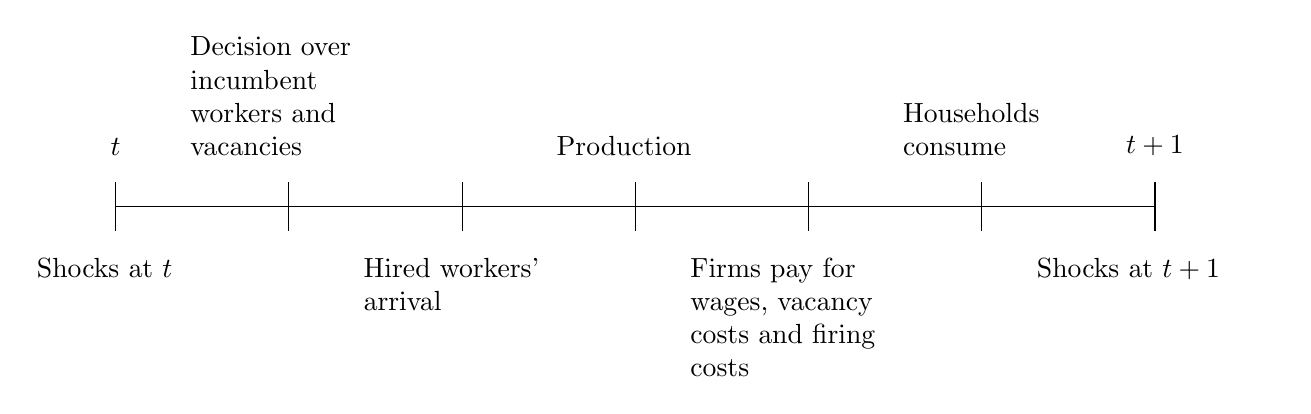
\begin{tikzpicture}[scale = 0.88]
%draw horizontal line
\draw (0cm,0cm) -- (15cm,0cm);
draw vertical lines
\foreach \x in {0, 2.5, 5, 7.5, 10, 12.5, 15}{
   \draw (\x,10pt) -- (\x,-10pt);
}
\draw (0,0) node[below=15pt, text width=2cm] {Shocks at $t$} node[above=15pt] {$t$};
\draw (2.5,0) node[above=15 pt, text width=2.5cm] {Decision over incumbent workers and vacancies};
\draw (5,0) node[below=15pt, text width=2.5cm] {Hired workers' arrival};
\draw (7.5,0) node[above=15pt, text width=2cm] {Production};
\draw (10,0) node[below=15pt, text width=3cm] {Firms pay for wages, vacancy costs and firing costs};
\draw (12.5,0) node[above=15pt, text width=2cm] {Households consume};
\draw (15,0) node[below=15pt, text width=3cm] {Shocks at $t+1$} node[above=15pt] {$t+1$};
\end{tikzpicture}
\end{center}
\label{fig:timing}
\caption{The timing of the economy}
\end{figure}

\paragraph{Vacancies} I depart from the literature when it comes to job creation. \citet{sala2009flexibility} assumes that job creation occurs through fixed-term contracts only; open-ended jobs all come from converted fixed-term jobs, which is counterfactual. As \citet{CAHUC200263} first did, \citet{SJOE:SJOE1715} assume that new matches face hiring restrictions. Firms are allowed to hire either through an open-ended or a fixed-term contract according to an exogenous probability. Otherwise, all hires would take place through fixed-term contracts. As roughly 20\% of hires are open-ended in France, different reasons than legal constraints on fixed-term hires explain open-ended hires.

Thereby, I assume that no constraints bind job creation. When paired with a worker, firms hire through a fixed-term contract or through an open-ended contract. They can also return searching for a worker and get the chance to be matched with another one on the next period. The present discounted value of a vacancy $V_t$ bears witness of these different options:

\begin{equation} \label{eq:def_v}
V_t = - \gamma + q \left( \theta_{t} \right) \int max \left[ J_{t}^{0,p} \left( z \right) , J_{t}^{f} \left( z \right) ,  \mathbb{E}_{t} \beta_{t,t+1} V_{t+1} \right] dG(z)
\end{equation}

where $\gamma$ is the cost of a vacancy, $J_{t}^{0,p}$ is the firm's surplus with a new open-ended match and $J_t^{0,f}$ is the firm's surplus with a new fixed-term match. The counterpart of these surpluses for continuing open-ended matches and continuing fixed-term matches are $J_{t}^{p}$ and $J_t^{f}$. The associated surpluses of workers are denoted $W$, while the total surpluses are denoted $S$. 

\paragraph{Surplus sharing}

I assume that wages are set each period by Nash bargaining. It is not realistic considering the evidence supporting rigidity in wages. In addition, wage flexibility seems inconsistent with the stickiness of retailers' prices. Still, I leave rigid wages for future research. Tractability motivates the use of Nash bargaining. It makes hiring and firing decisions jointly efficient and only dependent on the total surplus of a match. Denoting $\eta$ the worker's share of the match surplus, the sharing rules write

\begin{align}
&W_t^p \left( z_t \right) = \eta S_t^p \left( z_t \right) \label{eq:nash_p}\\
&W_t^{0,p} \left( z_t \right) = \eta S_t^{0,p} \left( z_t \right) \label{eq:nash_0p}\\
&W_t^f \left( z_t \right) = \eta S_t^f \left( z_t \right) \label{eq:nash_f}
\end{align}

Total surpluses verify

\begin{align}
S_t^p \left( z_t \right) &= J_t^p \left( z_t \right) - \left( V_t - F_t \right) + W_t^p \left( z_t \right) - U_t \label{eq:def_sp}\\
S_t^{0,p} \left( z_t \right) &= J_t^{0,p} \left( z_t \right) - V_t + W_t^{0,p} \left( z_t \right) - U_t \label{eq:def_s0p}\\
S_t^{f} \left( z_t \right) &= J_t^{f} \left( z_t \right) - V_t + W_t^{f} \left( z_t \right) - U_t \label{eq:def_sf}
\end{align}

where $U_t$ is the value of unemployment at the beginning of period $t$. The outside option of workers includes taking part in current period's market trades and take the unemployment benefit if no beneficial meeting occurred.

\begin{align}
U_t &= p\left( \theta_t \right) \int \max \left( W_t^{0,p} (z), W_t^f (z), U_t^0 \right) dG(z) + \left( 1 - p\left( \theta_t \right) \right)U_t^0 \label{eq:U} \\
U_t^0 &= b_t + \mathbb{E}_t \beta_{t, t+1} U_{t+1} 
\end{align}

where $b_t = \rho^b \overline{w_t} + h$ is the unemployed's flow of utility. It includes unemployment benefits as well as home production $h$. 

In \eqref{eq:def_sp}-\eqref{eq:def_sf}, note that the surplus of incumbent open-ended matches includes firing costs, while the one of new open-ended workers does not. In case of disagreement during wage bargaining, a newly paired worker goes back to the pool of job seekers and the firm does not pay firing costs. That way, I do not overstate the role of firing costs.

Now, I describe the open-ended and the fixed-term contract and the associated surpluses.

\paragraph{Open-ended contracts}

A continuing open-ended contract delivers the wage $w_{t}^{p}$ and stipulates a firing tax $F_t$. An open-ended match may separate with the exogenous probability $s$. In this case, the separation bears no cost. Otherwise, the firm chooses whether it keeps or lays off the worker regarding the idiosyncratic productivity of the match. An endogenous separation entails the payment of the firing cost and the opening of a new vacancy. Hence, a firm with an incumbent open-ended worker has the following surplus

\begin{align} \label{eq:def_jp}
J_t^p \left( z_{t} \right) = \phi_t A_t z_{t} - w_{t}^{p} \left( z_t \right) + \mathbb{E}_{t} \beta_{t,t+1} \left\{ (1-s) \int \max \left[ J_{t+1}^{p} \left( z \right), V_{t+1} - F_{t+1} \right] dG(z) + s V_{t+1} \right\}
\end{align}

An incumbent open-ended worker earns a wage and may leave with probability $s$. If he does not, he faces a productivity shock and the match may split if the latter shock is adverse enough. Laid-off or quitting workers go back to the job seekers' pool immediately and are therefore eligible to participate to the current's period firm-worker meetings. Otherwise, the match goes on.

\begin{equation} \label{eq:def_wp}
W_t^p \left( z_t \right) = w_{t}^{p} \left( z_t \right) + \mathbb{E}_{t} \beta_{t,t+1} \left\{ (1-s) \int \max \left[ W_{t+1}^p ( z ), U_{t+1} \right]  dG(z) + s U_{t+1} \right\}
\end{equation}

New open-ended workers have a different wage function $w_t^{0,p}$: their outside option does not include the payment of the firing cost in case of disagreement during the wage bargaining and the possibility to search for a new job in case of disagreement. After one-period, if there is no separation, a wage renegotiation occurs because idiosyncratic productivity changed. The firm pays firing costs if an endogenous split occurs. Otherwise, the surplus of incumbent open-ended contracts weighs in. 

\begin{align} \label{eq:def_j0p} 
J_t^{0,p} \left( z_{t} \right) &= \phi_t A_t z_{t} - w_{t}^{0,p} \left( z_t \right) + \mathbb{E}_{t} \beta_{t,t+1} (1-s) \left\{ \int_{z_{t+1}^p}^{+\infty} J_{t+1}^{p} \left( z \right) dG(z) - G\left(z_{t+1}^p\right) F_{t+1} + s V_{t+1} \right\}\\
W_t^{0,p} \left( z_t \right) &= w_{t}^{0,p} \left( z_t \right) + \mathbb{E}_{t} \beta_{t,t+1} \left\{ (1-s) \int \max \left( W_{t+1}^p ( z ), U_{t+1} \right) dG(z) + s U_{t+1} \right\}
\end{align} 

\paragraph{Fixed-term contracts} A fixed-term contract stipulates the wage function $w_{t}^{f}$. Fixed-term matches split with the exogenous probability $\delta$. I assume that fixed-term contracts yield a lower productivity than open-ended matches with a factor $\rho < 1$. I discuss this assumption in detail below. Firms value the immediate production net of the wage. As for the continuation value, it simply embeds the possibility of an exogenous separation shock.

\begin{equation} \label{eq:def_jf}
J_{t}^f \left( z_t \right) = \rho A_t z_t \phi_t - w_{t}^{f} \left( z_t \right) + \mathbb{E}_{t} \beta_{t,t+1} \left\{ \left( 1-\delta \right)  \int J_{t+1}^{f} \left( z \right) dG(z) + \delta V_{t+1} \right\}
\end{equation}

Fixed-term workers immediately value their wage. In case of separation, they can immediately indulge in labor market trades.

\begin{equation} \label{eq:def_wf}
W_{t}^f \left( z_t \right) = w_{t}^{f} \left( z_t \right) + \mathbb{E}_{t} \beta_{t,t+1} \left\{ \left( 1-\delta \right)  \int W_{t+1}^{f} \left( z \right) dG(z) + \delta U_{t+1} \right\}
\end{equation}

Using the different definitions of the firms' and the workers' surpluses, the total surpluses write\footnote{Detailed calculations are available in Appendix \ref{sec:nb_surplus}}

\begin{align}
\begin{split} \label{eq:sp}
S_t^p \left( z_t \right) &= A_t z_t \phi_t - b - \frac{\eta \gamma \theta_{t}}{1-\eta} + F_t - \mathbb{E}_t \beta_{t,t+1} (1-s) F_{t+1} \\
&+ \mathbb{E}_t  \beta_{t,t+1} (1-s) \int \max \left( S_{t+1}^p \left( z \right), 0 \right) dG(z)
\end{split}\\
S_t^{0,p} \left( z_t \right) &= S_t^p \left( z_t \right) - F_t\label{eq:s0p}\\
S_t^f \left( z_t \right) &= \rho A_t z_t \phi_t - b - \frac{\eta \gamma \theta_{t}}{1-\eta} + \rho \mathbb{E}_t \beta_{t,t+1} (1-\delta) \int S_{t+1}^f ( z ) dG(z)\label{eq:sf}
\end{align}

As intended, the surplus of continuing open-ended workers includes the firing cost in case of endogenous separation. This bolsters his threat point in Nash bargaining and pushes up his wage. The new open-ended workers does not benefit from this effect since a failure in the bargaining process does not entail the payment of $F_t$. The total surplus of fixed-term workers shows the productivity gap $\rho$ in the flows and the exogenous termination of the contract in the continuation value. Fixed-term contracts hit with a job destruction shock split regardless the productivity of the match.

Using the firms' surpluses, joint surpluses and the surplus sharing rules, wages verify

\begin{align}
w_t^p \left( z_t \right) &= \eta \left( A_t z_t \phi_t + F_t - E_t \beta_{t,t+1} (1-s) F_{t+1} + \gamma \theta_{t} \right) + (1-\eta) b_t \label{eq:wp}\\
w_t^{0,p} \left( z_t \right) &= \eta \left( A_t z_t \phi_t - E_t \beta_{t,t+1} (1-s) F_{t+1} + \gamma \theta_{t} \right) + (1-\eta) b_t\\
w_t^f \left( z_t \right) &= \eta \left( \rho A_t z_t \phi_t + \gamma \theta_{t} \right) + (1-\eta) b_t\\
\end{align}

The new open-ended worker is penalized with higher firing costs to compensate the future gains of wages in case of continuation. Moreover, labor market tightness increases the outside option of workers through the higher probability of finding a job. Wages increase with labor market tightness.

\subsection{Job creation and job destruction}

I assume there is free entry on vacancy posting.

\begin{equation}
V_t = 0 \label{eq:free_entry}
\end{equation}

The job creation condition stems from the free-entry condition \eqref{eq:free_entry} and the Bellman equation defining the present discounted value of an unfilled vacancy \eqref{eq:def_v}. Using the Nash-sharing rules \eqref{eq:nash_0p}-\eqref{eq:nash_f}, the job creation condition becomes

\begin{align*}
\frac{\gamma}{(1-\eta) q\left( \theta_t \right)} = \int max \left[ S_t^{0,p} \left( z \right) , S_t^{f} \left( z \right), 0\right] dG(z)
\end{align*}

The choice between fixed-term and open-ended contracts lies in the comparison of joint surpluses across contracts. Notice that $\partial S_t^{0,p} / \partial z_t = A_t \phi_t A_t > \rho A_t \phi_t = \partial S_t^{f} / \partial z_t$. Thus, there exists a productivity threshold $z_t^*$ above which open-ended contracts are preferable to fixed-term ones.

\begin{align*}
S_t^{0,p} \left( z_t^* \right) = S_t^{f} \left( z_t^* \right) 
\end{align*}

As a result, job creation with \eqref{eq:def_sp_lin} and \eqref{eq:def_sf_lin}, one finds that $z_t^*$ verifies

\begin{equation}
(1-\rho) z_t^* = z_t^c - \rho z_t^f \label{eq:zs}
\end{equation}

I also define the threshold $z_t^p$ below which an incumbent open-ended match splits. Similarly, fixed-term contracts become profitable when productivity exceeds $z_t^f$. I denote $z_t^c$ the analogous threshold for new open-ended contracts.

\begin{align} \label{eq:def_zp}
&S_t^p \left( z_t^p \right) = 0 \\
\label{eq:def_zf}
&S_t^{f} \left( z_t^f \right) = 0\\ \label{eq:def_zc}
&S_t^{0,p} \left( z_t^c \right) = 0
\end{align}

Joint surpluses are linear in $z_t$. I can rewrite them using \eqref{eq:def_zp}-\eqref{eq:def_zf}. 

\begin{align}
&S_t^p (z) = A_t \phi_t \left( z - z_t^p \right) \label{eq:def_sp_lin} \\
&S_t^f (z) = \rho A_t \phi_t \left( z - z_t^f \right) \label{eq:def_sf_lin}
\end{align}

Using \eqref{eq:sp}-\eqref{eq:def_zc} and with integrations by part, equations profitability thresholds.

\begin{align} \label{eq:zp}
\begin{split}
&A_t z_t^p \phi_t + F_t - \mathbb{E}_t \beta_{t,t+1} (1-s) F_{t+1} + \mathbb{E}_t  \beta_{t,t+1} (1-s) A_{t+1} \phi_{t+1} \int_{z_{t+1}^p}^{+\infty} \left( 1 -  G(z) \right) dG(z)\\
&= b_t + \frac{\eta \gamma \theta_{t}}{1-\eta}
\end{split} \\
&A_t \phi_t z_t^c = A_t \phi_t z_t^p + F_t \label{eq:zc} \\
&\rho A_t z_t^f \phi_t + \rho \mathbb{E}_t \beta_{t,t+1} (1-\delta) A_{t+1} \phi_{t+1} \left( \mathbb{E}z - z_{t+1}^f \right) = b_t + \frac{\eta \gamma \theta_{t}}{1-\eta} \label{eq:zf}\\
\end{align}

Using these thresholds and integrations by part, I rewrite the job creation condition.

\begin{align} \label{eq:jc}
\frac{\gamma}{(1-\eta) q\left( \theta_t \right) A_t \phi_t} = \int_{\max \left[ z_t^c, z_t^* \right]}^{+\infty} \left( 1-G(z) \right) dz + \rho \int_{z_t^f}^{\max \left[ z_t^c, z_t^* \right]} \left( 1-G(z) \right) dz
\end{align}

The following proposition sums up job creation.

\begin{proposition} \label{prop:jc} Given $\left( z_t^p, z_t^c, z_t^f, z_t^* \right)$,
\begin{itemize}
\item if $z_t^* \leq z_t^f \leq z_t^c$, job creation is carried out through open-ended contracts only. it occurs when $z \geq z_t^c$ as figure \ref{fig:oe_only} shows.

\begin{figure}[H]
\centering
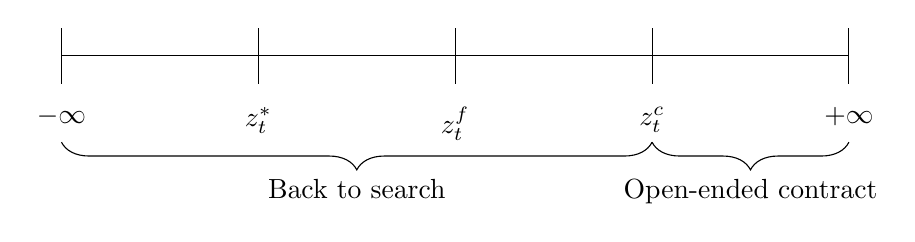
\begin{tikzpicture}[]
%draw horizontal line
\draw (0,0) -- (10cm,0);
%draw vertical lines
\foreach \x in {0,2.5,5,7.5,10}{
   \draw (\x cm, 10pt) -- (\x cm,-10pt);
}

%draw nodes
\draw (0,0) node[below=15pt,name = zbeg] {$-\infty$};
\draw (2.5cm,0) node[below=15pt,name = zs] {$z_t^*$};
\draw (5cm,0) node[below=15pt,name=  zf] { $z_t^f$};
\draw (7.5cm,0) node[below=15pt,name=  zc] { $z_t^c$};
\draw (10cm,0) node[below=15pt,name = zend] {$+\infty$};

\draw [decoration={brace,amplitude=10pt}, decorate] (zc.south) -- (zc.south -| zbeg.south) node [below = 10pt, pos=0.5] {Back to search};
\draw [decoration={brace,mirror,amplitude=10pt}, decorate] (zc.south) -- (zc.south -| zend.south) node [below = 10pt, pos=0.5] {Open-ended contract};
\end{tikzpicture}
\caption{\label{fig:oe_only} Open-ended hires only}
\end{figure}

\item Otherwise, necessarily, $z_t^c \leq z_t^f \leq z_t^*$: job creation is carried out through both open-ended contracts and fixed-term contracts. Fixed-term contracts are hired when $z \in ( z^f, z^* )$ and open-ended contracts are hired  when $z \in ( z^*, + \infty )$. Figure \ref{fig:dual_jc} sums it up.

\begin{figure}[H]
\centering
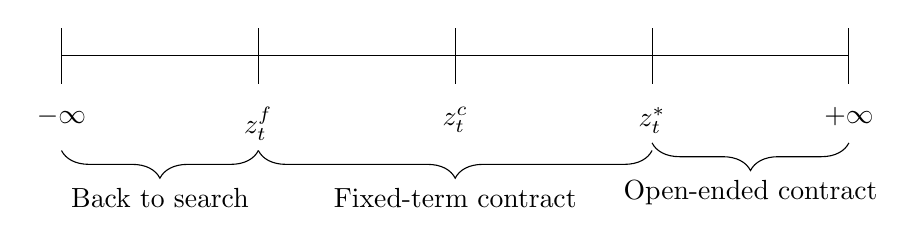
\begin{tikzpicture}[]
%draw horizontal line
\draw (0,0) -- (10cm,0);
%draw vertical lines
\foreach \x in {0,2.5,5.,7.5,10}{
   \draw (\x cm, 10pt) -- (\x cm,-10pt);
}

%draw nodes
\draw (0,0) node[below=15pt,name = zstart] {$-\infty$};
\draw (2.5cm,0) node[below=15pt,name=  zf] { $z_t^f$};
\draw (5cm,0) node[below=15pt,name=  zc] { $z_t^c$};
\draw (7.5cm,0) node[below=15pt,name = zs] {$z_t^*$};
\draw (10cm,0) node[below=15pt,name = zend] {$+\infty$};

\draw [decoration={brace,amplitude=10pt}, decorate] (zf.south) -- (zf.south -| zstart.south) node [below = 10pt, pos=0.5] {Back to search};
\draw [decoration={brace,mirror,amplitude=10pt}, decorate] (zf.south) -- (zf.south -| zs.south) node [below = 10pt, pos=0.5] {Fixed-term contract};
\draw [decoration={brace,mirror,amplitude=10pt}, decorate] (zs.south) -- (zs.south -| zend.south) node [below = 10pt, pos=0.5] {Open-ended contract};
\end{tikzpicture}
\caption{\label{fig:dual_jc} Dual job creation}
\end{figure}
\end{itemize}
\end{proposition}
\begin{proof}
See Appendix \ref{app:proofs}
\end{proof}

Demonstrating proposition \ref{prop:jc} follows the same steps as in \citet{rion:halshs-02331887}. However, the choice between open-ended contract and a fixed-term contract does not stem from the same mechanisms. Here, the trade-off opposes flexibility and productivity. An open-ended contract delivers a full productivity but may lead to the payment of firing costs if an adverse productivity shock hits. Thus, hiring an open-ended worker is worth it if productivity is high enough to overcome the expected firing costs. A fixed-term contract delivers a lower productivity, but it is shorter and separation costs zero. The option of hiring a fixed-term contract makes agents short-sighted: it pushes up the minimum productivity to hire an open-ended contract and tightens the hiring window for open-ended contracts.  

\citet{rion:halshs-02331887} is similar to the present model with two notable exceptions. Firstly, open-ended and fixed-term workers have the same productivity. Secondly, matches face i.i.d productivity shocks, whose occurrence follows a Poisson law. A new match with a high productivity chooses a contract to last as long as possible: it would be a pity to split before any productivity shock hits and to lose the advantage of a high productivity draw. Thus, on average, an open-ended contract lasts longer than a fixed-term contract and enables to lock up highly productive matches. A new match with a lower initial productivity may not find it optimal to face the risk of paying firing costs in the doldrums to secure current gains. In worst cases, going back to search is the best option. In the middle ground, though, fixed-term contracts are relevant; they enable both production and a quick return to search for a better match.

In this paper, productivity shocks no longer hit at random according to a memory-less Poisson law, which cuts out the incentive to secure the most productive matches through open-ended contracts.  When meeting, a firm and a worker know that the current productivity draw will last one period. They do not hope a high productivity draw to last forever. Thereby, Fixed-term contracts lose their role of median solution between producing and searching for more productive matches. One contract would be systematically preferred to the other without the contractual productivity gap. Still, the assumption that fixed-term contracts are \emph{per se} less productive than open-ended ones is not far-fetched. Fixed-term positions are mainly filled by low-skilled or inexperienced workers \citep{fontaine2016cdd} and benefit less from on-the-job training \citep{doi:10.1111/1467-8543.00106,10.1162/154247604323068041,Albert2005,10.1093/esr/jcs011}. \citet{doi:10.1111/ecin.12077} estimate that fixed-term workers are 20\% less productive than open-ended workers.

The main departure with \citet{sala2009flexibility} and \citet{SJOE:SJOE1715} is the appearance of the threshold $z_t^*$. The movements in thresholds $z_t^p$, $z_t^c$, $z_t^f$ and $z_t^*$ shape the behavior of the labor market and its fluctuations. If job creation involves both fixed-term and open-ended contracts --- as will be the case in my calibration --- then Figure \ref{fig:pdf} sums up the hiring and firing policies and the position of the thresholds if idiosyncratic productivity shocks are drawn from a log-Normal distribution.

\begin{figure}[H]
\begin{center}
\begin{tikzpicture}

\newcommand\zp{0.62}
\newcommand\zf{1.08}
\newcommand\zs{1.28}
\newcommand\sigz{0.2}

\begin{axis}[
clip=false,
height = 10cm,
width = 10cm,
xlabel = $z$,
ylabel = {},	
xmin = exp(\sigz^2)-3*\sigz,
xmax = exp(\sigz^2)+4*\sigz,
ymin = 0.,
ymax = 2.25,
axis lines = middle,
legend pos= outer north east,
xtick = {\zp,\zf,\zs},
xticklabels={$z^p$,$z^f$,$z^*$}
]

\addplot[color = black,ultra thick,samples=1000,domain = 0.25:2.] { exp(-0.5*ln(x)^2/(0.2^2)) / (x*0.2*sqrt(2*pi))} ;
\addplot [color = black,thick,dashed]  coordinates { (\zp,0.) (\zp,{exp(-0.5*ln(\zp)^2/(0.2^2)) / (\zp*0.2*sqrt(2*pi))} ) };
\addplot [color = black,thick,dashed]  coordinates { (\zf,0.) (\zf,{exp(-0.5*ln(\zf)^2/(0.2^2)) / (\zf*0.2*sqrt(2*pi))} ) };
\addplot [color = black,thick,dashed]  coordinates { (\zs,0.) (\zs,{exp(-0.5*ln(\zs)^2/(0.2^2)) / (\zs*0.2*sqrt(2*pi))} ) };
\draw [thick,decoration={brace,mirror,amplitude = 10pt},decorate] (axis cs:{exp(\sigz^2)-3*\sigz},0.) -- (axis cs:\zp,0.) node[midway, anchor=north west, yshift=-0.5cm, rotate = -45] {Firing open-ended contract};
\draw [thick,decoration={brace,mirror,amplitude = 10pt},decorate] (axis cs:\zf,0.) -- (axis cs:\zs,0.) node[midway, anchor=north west, yshift=-0.5cm, rotate = -45] {Hiring fixed-term contract};
\draw [thick,decoration={brace,mirror,amplitude = 10pt},decorate] (axis cs:\zs,0.) -- (axis cs:{exp(\sigz^2)+4*\sigz},0.) node[midway, anchor=north west, yshift=-0.5cm, rotate = -45] {Hiring open-ended contract};
\end{axis}
\end{tikzpicture}
\end{center}
\caption{The probability distribution function of idiosyncratic shocks and the location of thresholds}
\begin{flushleft}
\small The displayed pdf belongs to a log-Normal low with zero mean and standard deviation 0.2. \normalsize
\end{flushleft}
\label{fig:pdf}
\end{figure}

\subsection{Fiscal and monetary policy}

The government taxes households in order to provide for the unemployment benefits. The revenues from the firing tax get back to the government. Thus, the budget constraint of the government is

\begin{equation}
\tau_t + (1-s) G\left( z_t^p \right) n_t^p F_t = \rho^b \overline{w_t} u_t + g_t
\end{equation}

where $g_t$ is the government expenditure and follows the AR(1) log-process $log\left(g_t\right) = \left(1-\rho_g\right) log\left(\overline{g}\right) + \rho_g log\left( g_{t-1} \right) + \epsilon_t^g$, $\epsilon_t^g \sim \mathcal{N} \left( 0, \sigma_g^2 \right)$.

The monetary policy is decided in accordance with the Taylor rule

\begin{equation}
log\left( R_{t} / R \right) = \rho_R log\left( R_{t-1} / R\right) + \left( 1 - \rho_R \right) \left[ \rho_{\pi} \mathbb{E}_t log \left( \frac{P_{t+1}}{P_t} \right) + \rho_y log\left(\frac{y_t}{y}\right) \right] + \epsilon_t^m \label{eq:taylor}
\end{equation}

where $y$ is the steady-state output and $\epsilon_t^m \overset{iid}{\sim} \mathcal{N} \left( 0, \sigma_m^2 \right)$.

Fixed-term contracts are known to behave as buffers in front of workload fluctuations, as \citet{saint1996dual} documented. Thus, the case of indeterminacy in the Taylor rule and the subsequent appearance of sunspot equilibria may prove interesting. For the sake of simplicity, though, I shall restrain the present analysis to the determinate case with $\rho_{\pi} > 1$ and $\rho_y > 0$ and leave indeterminacy and its consequences on dual labor markets for future research.

\subsection{Aggregate values and the equilibrium}

This paragraph sums up the different conditions enabling an utter closing of the model. The employment values sum to the measure of households, namely 1.

\begin{equation}
n_t^p + n_t^f + u_t = 1
\end{equation}

$n_t^p$, $n_t^f$ and $u_t$ are the measures of open-ended employees, fixed-term employees and unemployed workers.

The aggregate stock of job-seekers includes the formerly unemployed households and the new entrants in the unemployment pool from the current period.

\begin{equation}
e_t = u_{t-1} + \delta n_{t-1}^f + \xi_t n_{t-1}^p
\end{equation}

The labor market tightness is the ratio between aggregate number of vacancies $v_t = \int_{0}^{1} v_{i,t} di$ and the number of job seekers.

\begin{equation*}
\theta_t = \frac{v_t}{e_t}
\end{equation*}

The employment variables drop by the job destruction flow and augment by the job creation flow.

\begin{align}
n_t^p &= \left( 1 - \xi_t \right) n_{t-1}^p + \mu_t^p e_t\\
n_t^f &= \left( 1 - \delta \right) n_{t-1}^f + \mu_t^f e_t
\end{align}

where $\mu_t^p = p\left( \theta_t \right) \left( 1- G\left( z_t^*\right)\right)$ and $\mu_t^f = p\left( \theta_t \right) \left( G\left( z_t^*\right)-G\left( z_t^f \right)\right)$ are the open-ended and fixed-term job-finding rates. $\xi_t = s + (1-s) G\left( z_t^p \right)$ is the the job destruction rate of open-ended contracts.

As for firms, the aggregate demand for final goods is

\begin{equation}
Y_t = c_t + g_t + \gamma v_t \label{eq:res_cons}
\end{equation}

The retailers face only one real marginal cost from the intermediate firms, which entails a unique equilibrium value for the optimal price-setting program, \emph{id est} $P_{i,t}^* = P_t^*$.

The market clearing condition for intermediate goods states that intermediate goods are produced by incumbent workers or new workers through either open-ended or fixed-term contracts. 

\begin{align*}
\int_{0}^{1} Y_{i,t} di &= A_t E_z \left[z \mid z \geq z_t^p \right] \left( 1 - \xi_t \right) n_{t-1}^p + \left( 1 - G\left( z_t^* \right)\right) q \left( \theta_t \right) v_t A_t E_z \left[z \mid z \geq z_t^* \right]\\
&+ \rho A_t \mathbb{E}_z \left[ z \right] \left( 1 - \delta \right) n_{t-1}^f + \rho \left( G\left( z_t^* \right) - G\left( z_t^f \right)\right) q \left( \theta_t \right) v_t A_t \mathbb{E}_z \left[z \mid z_t^* \geq z \geq z_t^f \right]
\end{align*}

Using the first order condition from the final good firm's program \eqref{eq:ret_dem}, I get

\begin{align}
\begin{split}
Y_t \Delta_t &= A_t E_z \left[z \mid z \geq z_t^p \right] \left( 1 - \xi_t \right) n_{t-1}^p + \left( 1 - G\left( z_t^* \right)\right) q \left( \theta_t \right) v_t A_t E_z \left[z \mid z \geq z_t^* \right]\\
&+ \rho A_t E_z \left[ z \right] \left( 1 - \delta \right) n_{t-1}^f + \rho \left( G\left( z_t^* \right) - G\left( z_t^f \right)\right) q \left( \theta_t \right) v_t A_t E_z \left[z \mid z_t^* \geq z \geq z_t^f \right] \label{eq:res_cons_int}
\end{split}
\end{align}

with $\Delta_t = \int_{0}^{1} \left( \frac{P_{i,t}}{P_t}\right)^{-\epsilon_t} di$ which measures price dispersion. \citet{yun1996nominal} demonstrated that the associated law of motion is

\begin{equation}
\Delta_t = (1-\psi) \left( \frac{P_t^*}{P_t} \right)^{-\epsilon_t} + \psi \left( \frac{P_t}{P_{t-1}} \right)^{\epsilon_t} \Delta_{t-1}
\end{equation}

while the price level follows

\begin{equation}
P_t = \left[ \psi P_{t-1}^{1-\epsilon_t} + (1-\psi) \left( P_t^* \right)^{1-\epsilon_t} \right]^{\frac{1}{1-\epsilon_t}} \label{eq:lm_price}
\end{equation}

Average wages pinpoint unemployment benefits as well as firing costs. Firing costs are a share of the average wage of incumbent open-ended workers. Denoting $\widetilde{w_t^p}$ the average wage of incumbent workers with open-ended contracts, firing costs verify

\begin{align}
F_t = \rho^F \widetilde{w_t^p}
\end{align}

The average wage of incumbent open-ended workers is simply the expected wage of open-ended matches with a productivity higher than the firing threshold.

\begin{align*}
\widetilde{w_t^p} &= \mathbb{E}_t \left[ w_t^p \left( z \right) \mid z \geq z_t^p\right]
\end{align*}

Using \eqref{eq:wp}, the average wage of incumbent open-ended workers boils down to

\begin{align}
\widetilde{w_t^p} &= \eta \left( A_t \phi_t \mathbb{E}_t \left[ z \mid z_t^p \leq z \right] + F_t - E_t \beta_{t,t+1} (1-s) F_{t+1} + \gamma \theta_{t} \right) + (1-\eta) b_t
\end{align}

The average wage of open-ended workers includes the wage that are not fired and with productivity higher than the firing threshold.

\begin{align*}
\overline{w_t^p} &= \frac{\left( 1-\xi_t \right) n_{t-1}^p \mathbb{E}_t \left[ w_t^p \left( z \right) \mid z \geq z_t^p\right] + \mu_t^p e_t \mathbb{E}_t \left[ w_t^{0,p} \left( z \right) \mid z \geq z_t^*\right]}{n_t^p}\\
\overline{w_t^f} &= \frac{\left( 1-\delta \right) n_{t-1}^f\mathbb{E}_t \left[ w_t^f \left( z \right) \right] + \mu_t^f e_t \mathbb{E}_t \left[ w_t^{f} \left( z \right) \mid z_t^f \leq z \leq z_t^*\right]}{n_t^f}\\
\end{align*}

Given the path of exogenous shocks $\left\{ \epsilon_t^A, \epsilon_t^\mu, \epsilon_t^g, \epsilon_t^m \right\}_{t=0}^{+\infty}$, laws of motions of exogenous shocks $\left\{ A_t, \mu_t , g_t \right\}_{t=0}^{+\infty}$ and initial values for the state variables $\left\{ R_{-1}, n_{-1}^p, n_{-1}^f, \Delta_{-1}, P_{-1} \right\}$, the equilibrium sums up into the set of endogenous variables $\left\{ R_t, c_t, Y_t, n_t^p, n_t^f, u_t, \Delta_t, z_t^p, z_t^c, z_t^f, z_t^*, \theta_t, \phi_t, v_t, P_t, P_t^*, b_t, F_t, \overline{w_t^p}, \overline{w_t^f}, \widetilde{w_t^p} \right\}_{t=0}^{+\infty}$ pinned down by equations \eqref{eq:euler_eq}, \eqref{eq:price_eq}, \eqref{eq:zp}-\eqref{eq:zf}, \eqref{eq:zs} and \eqref{eq:taylor}-\eqref{eq:lm_price}. 